\chapter{Application}
\label{application}
%#############################################################################################

In this chapter, we are trying to apply the algorithms that are described and implemented in Chapter~\ref{implementation} to various datasets: \textit{usps}, \textit{banana}, \textit{fishbowl}, \textit{swissroll} and \textit{flatroll}.

\section{Assignment 4: PCA}
\label{assignment4}

This assignment asks us to apply \textit{PCA} to the \textit{usps} data set and visualizing the results. The \textit{usps} data set consists of 2007 images with the dimension of \textit{16 x 16}. The images are hand-written digits of zero to nine, which can be viewed as classes. Firstly, i separate the data set according to each digit into ten classes and then applied \textit{PCA} to each class. The \textit{PCA} was applied to the original data set and noisy data set.

\subsection{Original Data Set}
\label{ass4:original}

PCA was applied to each class and then the results were visualized. As depicted in Figure~\ref{fig:pcaOriginal05} and \ref{fig:pcaOriginal69}, the following were visualized:

\begin{itemize}
	\item All principle values (as bar plot).
	\item The largest 25 principal values (as bar plot).
	\item The first 5 principal directions (as images).
\end{itemize}

From the visualization, it can be obtained that the information of the data set is only represented by a small subset of principal components, about five to ten components. 

\begin{figure}[h!]
	\centering
	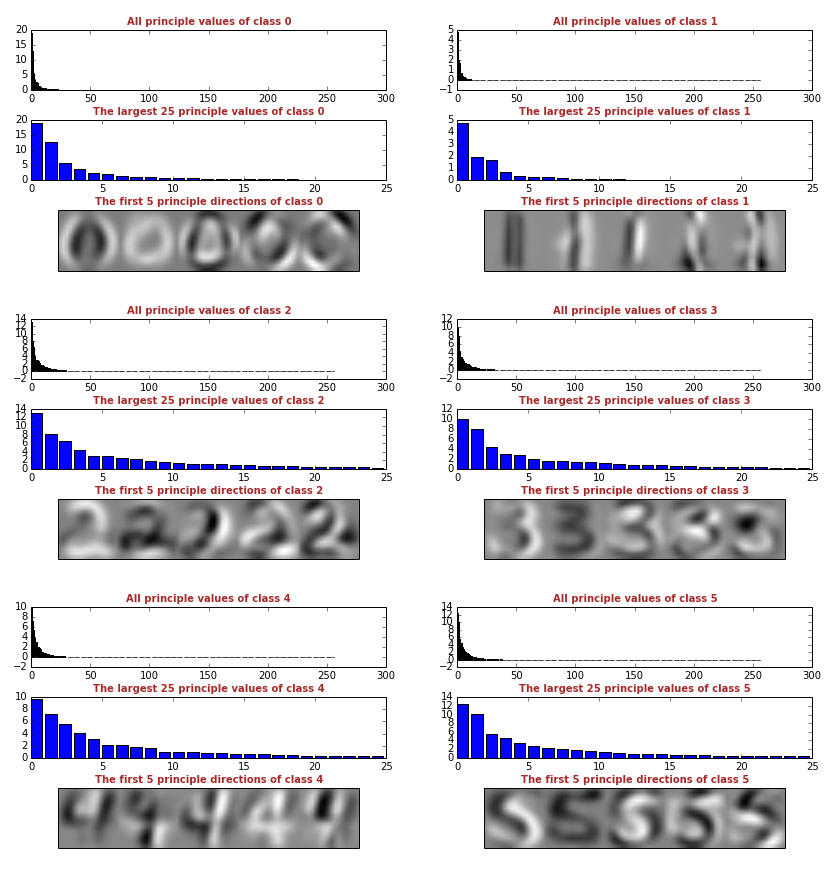
\includegraphics[scale=0.4983]{normalpca_0-5}
	\caption{Principal components of usps original data set for class 0 - 5}
	\label{fig:pcaOriginal05}
\end{figure}

\begin{figure}[h!]
	\centering
	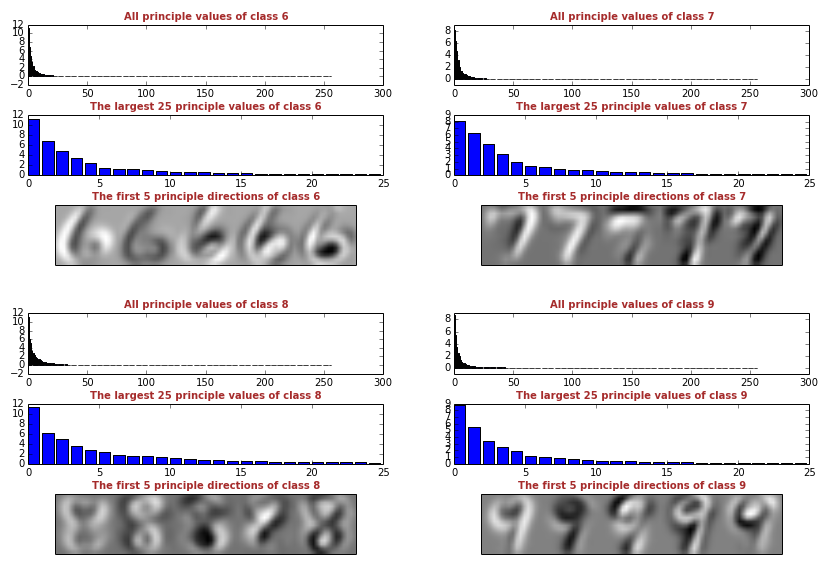
\includegraphics[scale=0.4983]{normalpca_6-9}
	\caption{Principal components of usps original data set for class 6 - 9}
	\label{fig:pcaOriginal69}
\end{figure}

\subsection{Noisy Data Set}
\label{ass4:noisy}

To make it more challenging, some noised are added to the original data set. There are three noise scenarios: \textit{low gaussian noise}, \textit{high gaussian noise} and \textit{outliers}.

For the \textit{low gaussian noise}, standard deviation used to generate the noise is 0.25, whereas for \textit{high gaussian noise} and \textit{outliers}, standard deviations of 0.55 and 1.25 are used, respectively. The same steps as in Subsection~\ref{ass4:original} are performed for all noisy data sets. The visualization is depicted in Figure~\ref{fig:pcaModerate05} to \ref{fig:pcaExtreme69}.

\begin{figure}[h!]
	\centering
	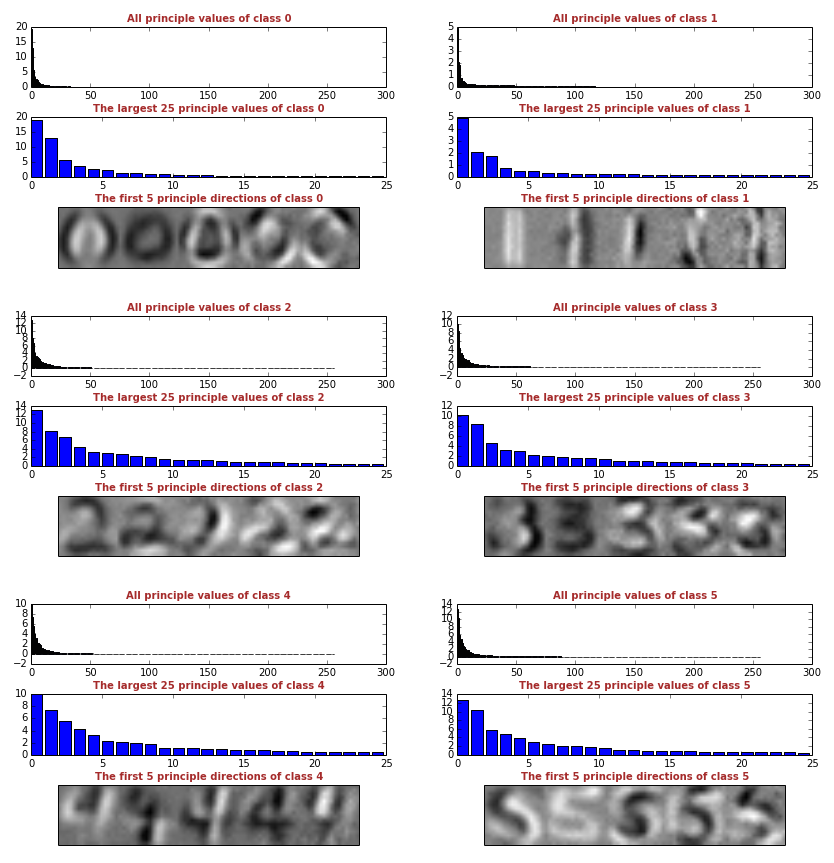
\includegraphics[scale=0.4983]{moderately_noisy_0-5}
	\caption{Principal components of moderately noisy data set for class 0 - 5}
	\label{fig:pcaModerate05}
\end{figure}

\begin{figure}[h!]
	\centering
	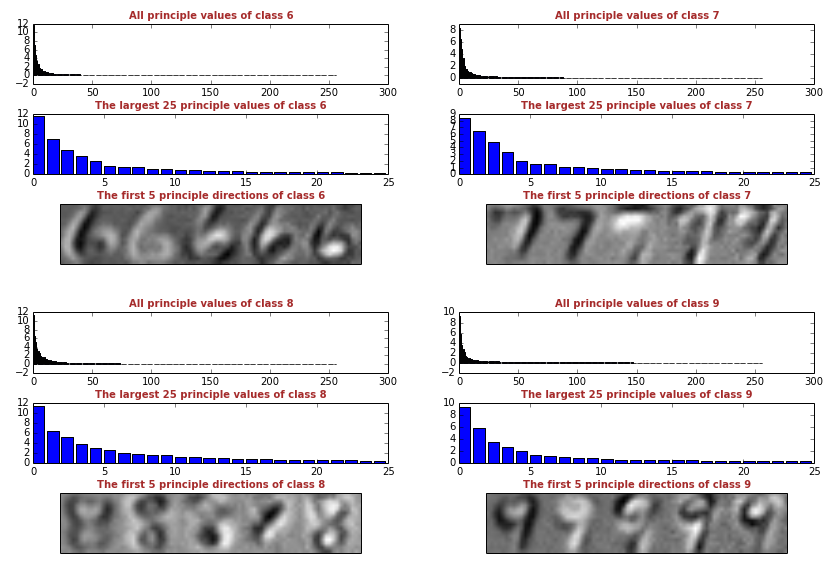
\includegraphics[scale=0.4983]{moderately_noisy_6-9}
	\caption{Principal components of moderately noisy data set for class 6 - 9}
	\label{fig:pcaModerate69}
\end{figure}

\begin{figure}[h!]
	\centering
	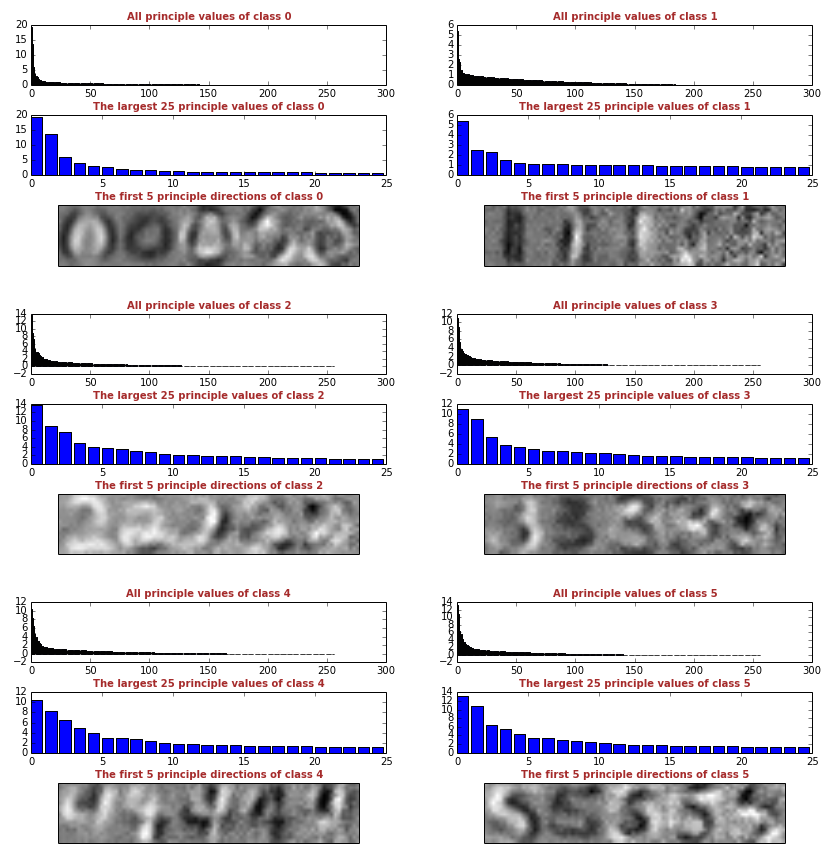
\includegraphics[scale=0.4983]{very_noisy_0-5}
	\caption{Principal components of very noisy data set for class 0 - 5}
	\label{fig:pcaVery05}
\end{figure}

\begin{figure}[h!]
	\centering
	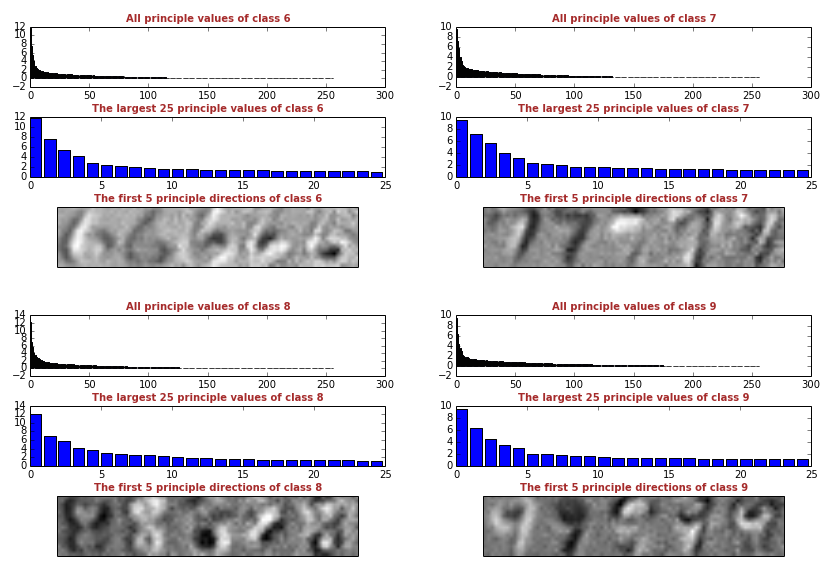
\includegraphics[scale=0.4983]{very_noisy_6-9}
	\caption{Principal components of very noisy data set for class 6 - 9}
	\label{fig:pcaVery69}
\end{figure}

\begin{figure}[h!]
	\centering
	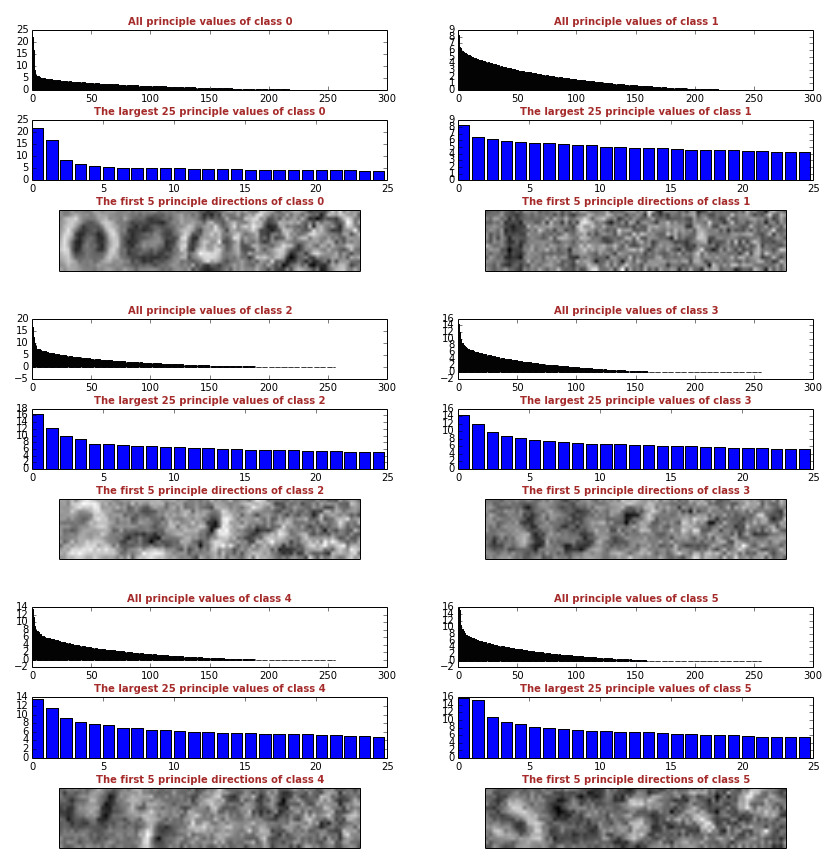
\includegraphics[scale=0.4983]{extremely_noisy_0-5}
	\caption{Principal components of extremely noisy data set for class 0 - 5}
	\label{fig:pcaExtreme05}
\end{figure}

\begin{figure}[h!]
	\centering
	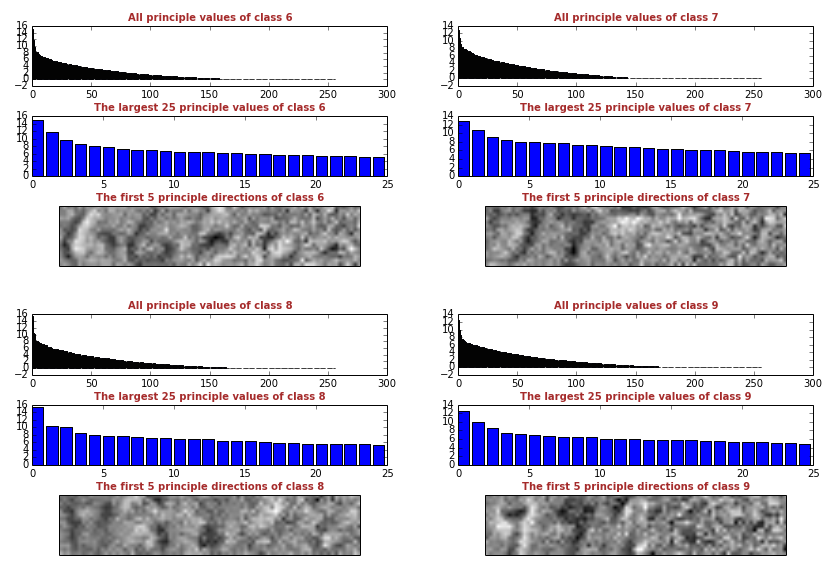
\includegraphics[scale=0.4983]{extremely_noisy_6-9}
	\caption{Principal components of extremely noisy data set for class 6 - 9}
	\label{fig:pcaExtreme69}
\end{figure}

It can be obtained that the information of the data set is now represented by a bigger number of principal components. The noisier a data set is, the bigger the number of principal components is needed to represent the information of the data set.

Figure~\ref{fig:pcaExamples} shows ten images of the original data, noisy data, and their reconstruction (denoised) data using \textit{PCA}. The number of components \textit{m} used for \textit{moderately} noisy images is 11, for \textit{very} noisy images is 75 and for \textit{extremely} noisy images is 150.

\begin{figure}[h!]
	\centering
	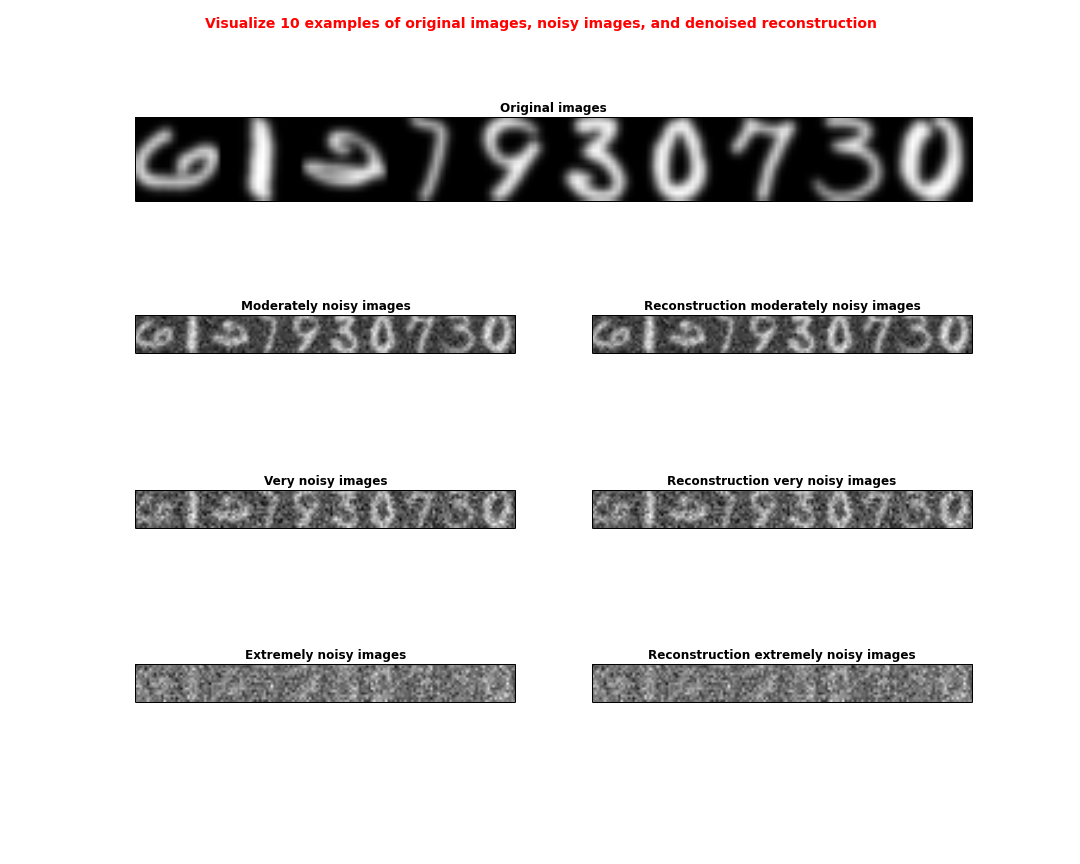
\includegraphics[scale=0.4983]{pcaexamples}
	\caption{Examples of some original, noisy and reconstruction images}
	\label{fig:pcaExamples}
\end{figure}

%#############################################################################################
\section{Assignment 5: Outlier Detection Using $\gamma$-Index}
\label{assignment5}

In this assignment, the $\gamma$-index method is utilized to detect outliers and applied it to the \textit{banana} data set. The positive class of the data set is used as \textit{inliers}, to which the negative class is added as outliers. The $\gamma$-index is then used to detect outliers with contamination rates of 1\%, 5\%, 10\% and 25\% relative to the positive class. Figure~\ref{fig:bananacomplete} shows the complete original data set, both positive and negative class, whereas Figure~\ref{fig:bananacontaminated} shows the contaminated data set.

\begin{figure}[h!]
	\centering
	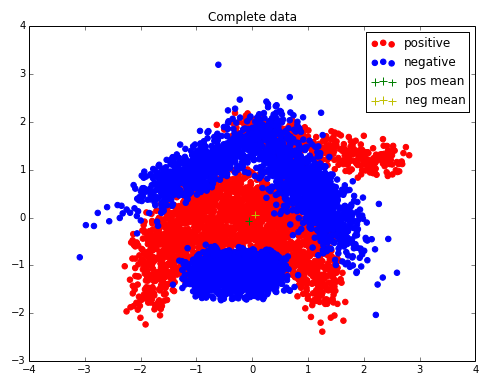
\includegraphics[scale=0.4983]{banana_complete}
	\caption{Both positive and negative of banana data set, including the mean of both classes}
	\label{fig:bananacomplete}
\end{figure}

\begin{figure}[h!]
	\centering
	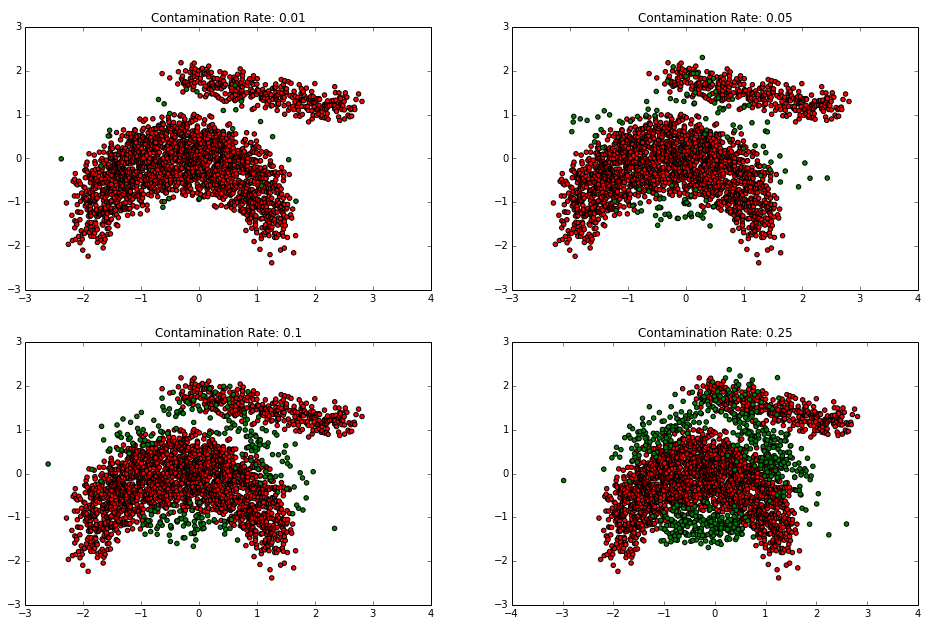
\includegraphics[scale=0.4983]{banana_contaminated}
	\caption{Contaminated banana data set with contamination rate of 1\%, 5\%, 10\% and 25\%}
	\label{fig:bananacontaminated}
\end{figure}

There are three methods that should be used to detect the outliers: (a) the $\gamma$-index with $k=3$, (b) the $\gamma$-index with $k=10$ and (c) the distance to the mean for each data point. All of the methods are then applied to the four contamination rates mentioned above. After that, the \textit{AUC} (area under the \textit{ROC}) should be calculated. Figure~\ref{fig:gammaboxplots} shows the boxplots that visualize the distribution of the \textit{AUC} values.

\begin{figure}[h!]
	\centering
	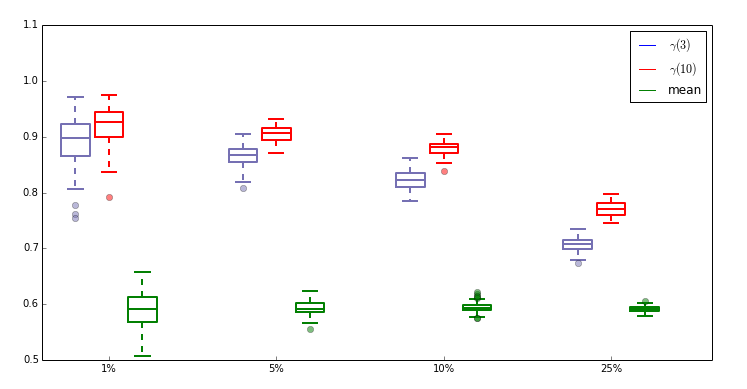
\includegraphics[scale=0.5583]{gamma_boxplots}
	\caption{Boxplots visualizing the distribution of the \textit{AUC} values}
	\label{fig:gammaboxplots}
\end{figure}

The boxplots show that the method using the distance to the mean for each data point performed quite bad, while both of the $\gamma$-index methods performed very well, especially for the data set with lower contamination rates. The $\gamma$-index with $k=10$ performed slightly better than the $\gamma$-index with $k=3$.


%#############################################################################################

\section{Assignment 6: LLE}
\label{assignment6}

In this assignment \textit{LLE} should be applied to the data sets \textit{fishbowl}, \textit{swissroll} and \textit{flatroll} using appropriate values for the parameters.

\subsection{Flatroll Data Set}
\label{ass6:flatroll}

For the \textit{flatroll} data set, it is quite easy to find the appropriate values for the parameters. Figure~\ref{fig:lleflatroll} shows the \textit{flatroll} data set and its resulting embedding using \textit{knn} rule with $k=12$ and regularization parameter $tol=1e-3$. The resulting embedding is quite good.

\begin{figure}[h!]
	\centering
	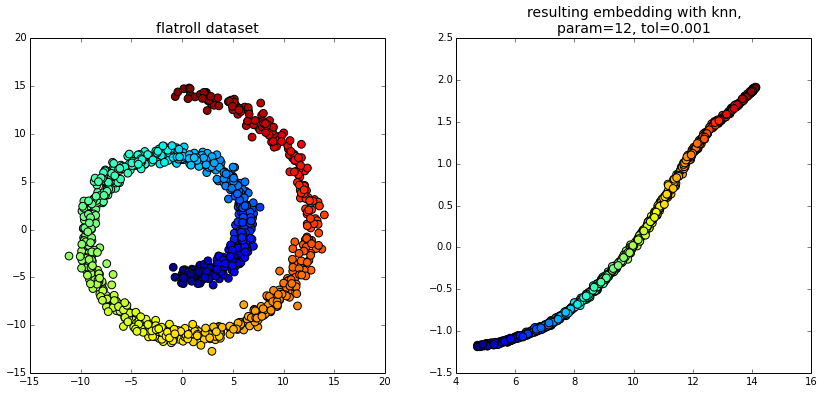
\includegraphics[scale=0.4983]{flatroll}
	\caption{Visualization of \textit{flatroll} data set and its resulting embedding}
	\label{fig:lleflatroll}
\end{figure}

\subsection{Swissroll Data Set}
\label{ass6:swissroll}

For the \textit{swissroll} data set, it is already quite hard to find the appropriate values for the parameters. Figure~\ref{fig:lleswissroll} shows the visualizationof the \textit{swissroll} data set and its resulting embedding using \textit{eps-ball} with $\epsilon=5.7$ and regularization parameter $tol=2.8e-5$. I cannot find the appropriate parameters.

\begin{figure}[h!]
	\centering
	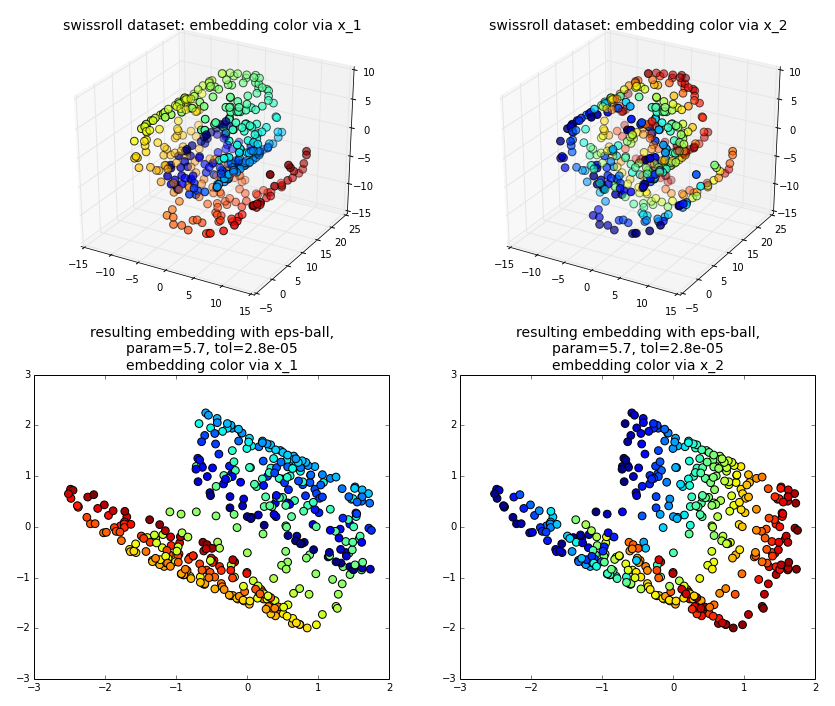
\includegraphics[scale=0.4983]{swissroll}
	\caption{Visualization of \textit{swissroll} data set and its resulting embedding}
	\label{fig:lleswissroll}
\end{figure}

\subsection{Dense Fishbowl Data Set}
\label{ass6:densefishbowl}

For the \textit{dense fishbowl} data set, i use \textit{knn} with $k=7$ and regularization parameter $tol=1e-5$. Figure~\ref{fig:lledensefishbowl} shows the visualization and its resulting embedding.

\begin{figure}[h!]
	\centering
	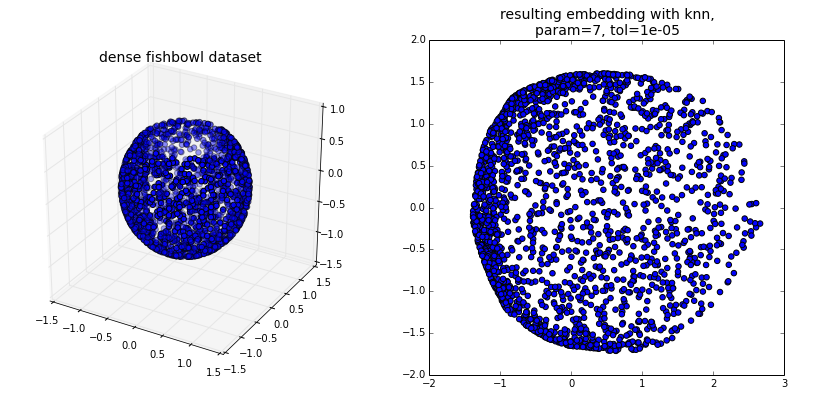
\includegraphics[scale=0.4983]{fishbowl_dense}
	\caption{Visualization of \textit{dense fishbowl} data set and its resulting embedding}
	\label{fig:lledensefishbowl}
\end{figure}

\subsection{Fishbowl Data Set}
\label{ass6:fishbowl}

For the \textit{fishbowl} data set, it is also really difficult to find the appropriate parameters. I cannot find them. Figure~\ref{fig:llefishbowl} shows the visualization of the \textit{fishbowl} data set and its resulting embedding using \textit{knn} with $k=14$ and regularization parameter $tol=4e-8$.

\begin{figure}[h!]
	\centering
	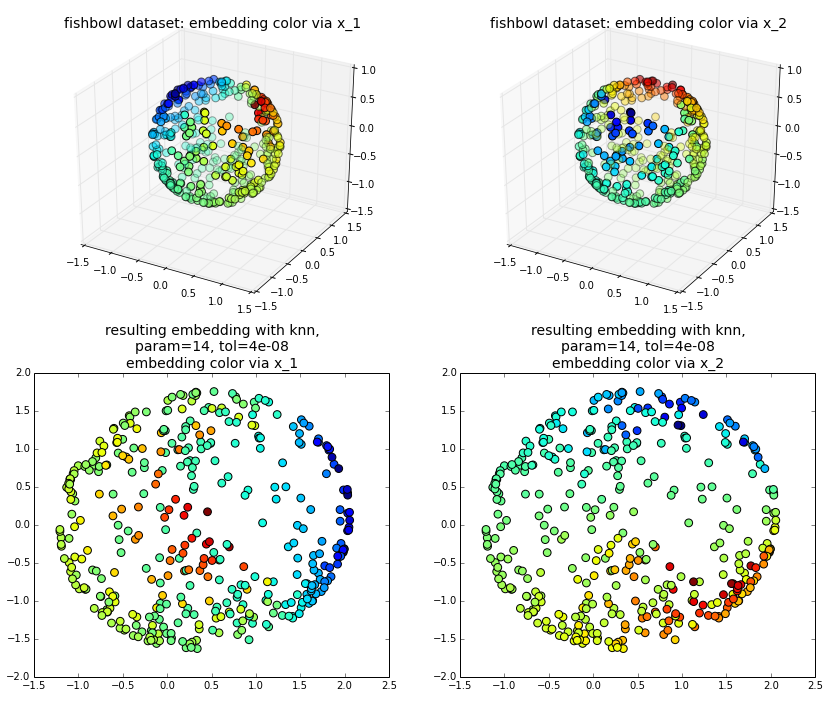
\includegraphics[scale=0.4983]{fishbowl}
	\caption{Visualization of \textit{fishbowl} data set and its resulting embedding}
	\label{fig:llefishbowl}
\end{figure}

%#############################################################################################

\section{Assignment 7: LLE With Noise}
\label{assignment7}

In the last assignment of this problem set, \textit{LLE} has to be applied to noisy \textit{flatroll} data set. Two gaussian noise were added to the data set, with variance 0.2 and 1.8, respectively. After that, both noisy data sets should be unrolled using \textit{knn} with a good value of \textit{k} and a value which is obviously too large. Figure~\ref{fig:llenoisy} depicts the two noisy images and their resulting embedding. It can be obtained that the noisy data set with big variance(1.8) is not very good unrolled.

\begin{figure}[h!]
	\centering
	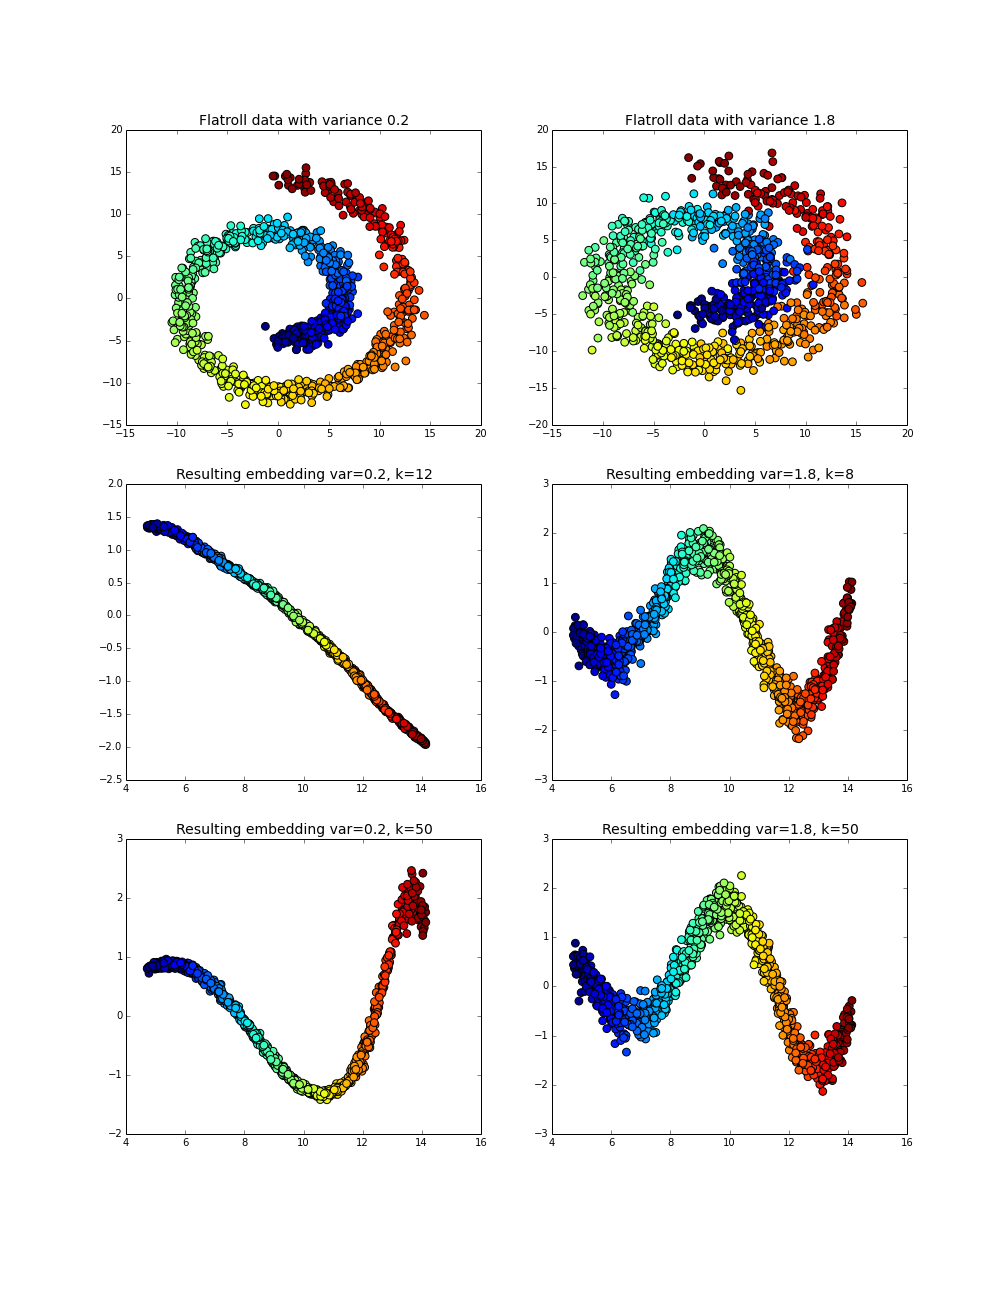
\includegraphics[scale=0.4983]{lle_noise}
	\caption{Visualization of two noisy \textit{flatroll} data set and their resulting embedding}
	\label{fig:llenoisy}
\end{figure}

